\section{Simulation study}\label{sec:simulation}
% Scale a table down (never up) to the line width.
\providecommand{\simfit}[1]{\resizebox{\ifdim\width>\linewidth\linewidth\else\width\fi}{!}{#1}}

Every number in this section comes from synthetic worlds with known ground truth. No real incident or record is used. The study asks six questions.
\begin{enumerate}[({Q}1)]
  \item How do the estimators of \cref{sec:identification,sec:models} behave under capture heterogeneity and referral, and does provenance recoding (\cref{prop:referral}(c)) remove the referral bias?
  \item Do the sensitivity bands of \cref{cor:bounds} contain the true dark figure?
  \item Does the linkage correction of \cref{cor:linkcorrect} work when its own model, LE (\cref{def:link-le}), generates the errors?
  \item Does it work when records carry realistic noise and are linked by Fellegi--Sunter EM?
  \item Does multiple imputation over linkage draws improve on a single linkage?
  \item Has the latent-class sampler converged at the settings we used?
\end{enumerate}
Q3 and Q4 are kept apart on purpose. In the record-level scenarios the records carry attribute noise and are linked by FS-EM, and LE is used nowhere in generating them. LE enters only through the correction, which is therefore tested under misspecification. A separate table-level scenario generates the errors by LE itself. The results are from the second run of the study, made after a code audit; \cref{app:simdetails} lists what changed from the first run, together with the full configurations, seeds, software versions, runtimes and reproduction commands.

\subsection{Design}\label{sec:sim-design}

\paragraph{Synthetic worlds.} Each world has $N=2000$ incidents. An incident has a date in one year (a quarter of the incidents fall in three two-week ``flashpoint'' spikes), an hour, one of 30 counties on a $6\times5$ grid, an offence type, a target and a venue string built from generic word lists. Four lists record the incidents: police, an NGO audit, a community security organisation and a campus or self-report portal ($K=4$). Capture follows one of three models.
\begin{itemize}
  \item \emph{Independent capture.} List $k$ records each incident with probability $p_k$, where $\bm p=(0.2725,0.305,0.2275,0.2075)$.
  \item \emph{Latent classes.} Each incident belongs to one of three reportability classes, ``visible'', ``moderate'' and ``low visibility'', with weights $(0.15,0.35,0.50)$. Given the class, the lists record independently, with probabilities between $0.30$ and $0.80$ in the visible class and between $0.06$ and $0.15$ in the low-visibility class (\cref{tab:sim-capture}). This is \eqref{eq:lcmcr} with three classes, so LCMCR is correctly specified, and $\bm p$ above is its marginal.
  \item \emph{Latent classes with covariates.} Class membership depends on the offence type, and type, target and campus location shift the logit capture probabilities. For instance, campus incidents are less likely to reach the police and more likely to reach the portal.
\end{itemize}
Referral (\cref{prop:referral}) is added by letting the NGO ingest each police-recorded incident with probability $q$. Every ingested record carries a provenance flag.

\paragraph{Records and linkage.} Every capture produces a record. At noise level $\nu$, records carry list-specific date lags and gross date errors, county errors and coarsening, type relabelling across four list vocabularies, typos, dropped words and missing values in the venue string, hour errors, and within-list duplicates (probability $0.04\nu$ per record). All rates scale with $\nu$, and $\nu=0$ gives clean records (\cref{app:sim-noise}). The records are then linked as in lines 1--2 of \cref{alg:pipeline}.
\begin{itemize}
  \item \emph{Blocking.} Candidate pairs lie in the same or adjacent counties and are at most 14 days apart.
  \item \emph{Comparison.} Comparison vectors record agreement on date, hour, county, harmonised type and venue (Jaro--Winkler). ``Missing'' is a level of its own.
  \item \emph{FS-EM.} A three-class model (match, related non-match, unrelated non-match) relaxes conditional independence for distinct incidents at the same venue \citep{larsen2001}.
  \item \emph{Linking.} After within-list deduplication, a greedy point linkage merges candidate pairs in decreasing order of the posterior match probability $\pi\ge0.5$, with at most one record per list in each cluster.
\end{itemize}
The error rates $(\delta,\varepsilon)$ of the point linkage are estimated by the random audit of \cref{prop:link-audit}. The audit draws $B=300$ candidate pairs, Neyman-allocated over strata of link status and posterior match probability, reveals the truth for each sampled pair, and computes $(\hat\delta,\hat\varepsilon)$ by \eqref{eq:link-psi}. Its estimand is defined on the candidate-pair frame, so true matches outside every block are invisible to it. It is not the targeted review of \cref{alg:review}, and reviewed links are not fixed.

\begin{table}[t]
\centering
\caption{Simulation scenarios (synthetic data). $R$: replicates per level; in parentheses, the replicates on which LCMCR is also run.}\label{tab:sim-design}
\small
\begin{tabular}{@{}llllll@{}}
\toprule
Scen. & Capture & Referral $q$ & Noise $\nu$ & $R$ & Purpose \\
\midrule
S1 & independent & 0 & 0 & 100 (10) & baseline \\
S2 & latent classes & 0 & 0 & 100 (25) & heterogeneity (Q1, Q6) \\
S3 & independent & 0.5 & 0 & 100 (10) & referral (Q1) \\
S4 & latent classes + covariates & 0 & 1 & 100 (25) & realistic linkage (Q1, Q4--Q6) \\
S5 & independent & 0 & 0, 0.25, 0.5, 1, 1.5, 2 & 40 per $\nu$ & linkage error (Q4, Q5) \\
S6 & \multicolumn{4}{l}{closed form $\widehat n_{\zero}(\omega)$ on the oracle tables of S1--S4} & sensitivity bands (Q2) \\
S7 & independent & 0, 0.25, 0.5, 0.75, 1 & oracle tables & 200 per $q$ & provenance recoding (Q1) \\
S8 & independent, table level & 0 & LE: $\delta\in\{0.05,0.1,0.2\}$, & 200 per cell & LE model holds (Q3) \\
 & & & \phantom{LE: }$\varepsilon\in\{0,0.02,0.05\}$ & & \\
\bottomrule
\end{tabular}
\end{table}

\paragraph{Scenarios.} \Cref{tab:sim-design} lists them. S6 reuses the oracle tables of S1--S4, and S7 analyses oracle tables only. S8 bypasses records. It draws a true table under independent capture and applies the LE model itself, incident by incident, on a $3\times3$ grid of $(\delta,\varepsilon)$, so the model behind \cref{cor:linkcorrect} holds exactly. The rates are then estimated by a simulated random audit of the LE linkage, with 200 records for $\delta$ and 100 linked edges for $\varepsilon$.

\paragraph{Estimators.} We compare five estimators:
\begin{itemize}
  \item LP: Lincoln--Petersen on police and NGO, in Chapman's form \citep{chapman1951} (\cref{thm:closed}(c));
  \item CF: the closed form of \cref{thm:closed} at $\omega=0$, with the interval of \cref{rem:id-intervals};
  \item BMA: model averaging over the 64 hierarchical log-linear models with all main effects and any subset of two-way interactions, with BIC weights and model-averaged Wald intervals \citep{turek2012};
  \item Chao's estimator (\cref{thm:chao});
  \item LCMCR: \eqref{eq:lcmcr} with $J^\star=10$ and the priors of \cref{sec:models-lcmcr}, reporting the posterior median and the equal-tailed interval.
\end{itemize}

\paragraph{Pipelines.} Each estimator is applied to the capture table produced by one of the following pipelines.
\begin{itemize}
  \item \emph{Oracle}: the true linkage.
  \item \emph{Naive}: the point linkage.
  \item \emph{LE-corrected}: \cref{cor:linkcorrect}(ii) applied to the naive table with the audit rates $(\hat\delta,\hat\varepsilon)$. The interval of the inner estimator is widened by $v_{\mathrm{link}}$ of \cref{cor:linkcorrect}(i), computed by the delta method through the Jacobian of the LE operator. For LCMCR, one chain is run on each of four imputed tables and the draws are pooled. A second interval also adds the audit variance of \cref{cor:linkcorrect}(iii). The audit samples the same linkage, so this sum is conservative (\cref{rem:link-sameaudit}).
  \item \emph{Three diagnostic variants of the correction.}
  \begin{itemize}
    \item \emph{Realised rates}: the realised rates of the point linkage replace the audit estimates. This separates misspecification of LE from audit error.
    \item \emph{The $\varepsilon=0$ variant} uses $(\hat\delta,0)$. We added it after the first run had shown the full correction failing, so it is \emph{post hoc}.
    \item \emph{Best-fit LE} uses the rates $(\delta^\ast,\varepsilon^\ast)$ that minimise a Pearson distance between $\Lop_{\delta,\varepsilon}(\bm t)$ and the naive table, where $\bm t$ is the oracle table. It is \emph{infeasible}, because it uses the truth. It shows the best that any scalar pair $(\delta,\varepsilon)$ can do.
  \end{itemize}
  \item \emph{MI}: twenty draws from a single-record Gibbs sampler over partitions with at most one record per list in each cluster. The sampler targets the plug-in Fellegi--Sunter pairwise posterior, with $m$ and $u$ fixed at their FS-EM values and candidate pairs with $\pi<10^{-3}$ truncated. These are approximate draws for the empirical-Bayes variant of line~5 of \cref{alg:pipeline}, not draws from a fully Bayesian linkage posterior. LP, CF, BMA and Chao are combined by Rubin's rules \citep{rubin1987} on $\log(\Nhat-c)$, where $c$ is a lower offset common to all draws, such as the smallest number of recorded incidents (\cref{prop:totalvar}(iv), \cref{app:sim-mi}). LCMCR pools one chain on each of the first four draws.
\end{itemize}

\paragraph{Metrics.} The primary metric is the median over replicates of the relative bias $(\Nhat-N)/N$. We also report means, but a few ``blow-ups'' ($\Nhat>5N$) can dominate them, so blow-ups are counted. Coverage is that of nominal $95\%$ intervals for the realised $N$. The Monte Carlo standard error (MCSE) of a coverage $c$ is $\{c(1-c)/R\}^{1/2}$. At $c=0.95$ it is $0.022$ for $R=100$, $0.015$ for $R=200$, $0.034$ for $R=40$, $0.044$ for $R=25$ and $0.069$ for $R=10$. Medians carry a distribution-free MCSE (\cref{app:sim-seeds}).

\subsection{Results}\label{sec:sim-results}

\begin{figure}[t]
\centering
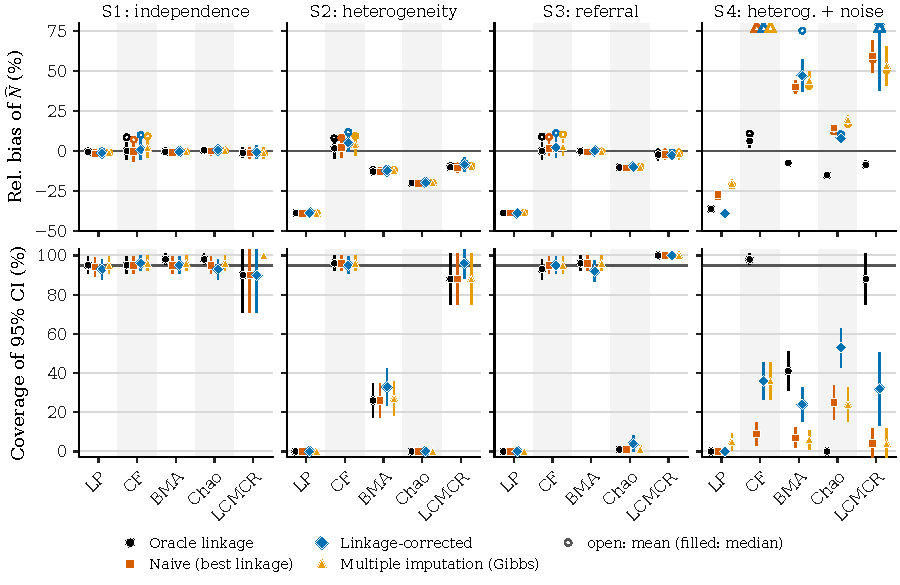
\includegraphics[width=6in]{figures/fig-sim-bias-coverage.pdf}
\caption{Synthetic data, scenarios S1--S4. Top: median relative bias of $\Nhat$ (filled; bars $\pm2$ MCSE) and mean relative bias (open). Bottom: coverage of nominal $95\%$ intervals (bars $\pm2$ MCSE). Triangles on the upper edge mark values beyond the axis. Linkage-corrected: LE correction with audit rates, interval with $v_{\mathrm{link}}$. $R=100$; LCMCR on 10 (S1, S3) or 25 (S2, S4) replicates.}\label{fig:sim-bias-coverage}
\end{figure}

\begin{table}[t]
\centering
\caption{Synthetic data, scenarios S1--S4. Median (MAD): median relative bias of $\Nhat$ in $\%$, with $1.4826\times$ the median absolute deviation in percentage points. Mean: mean relative bias in $\%$; the superscript counts replicates with $\Nhat>5N$. Cov.: coverage of nominal $95\%$ intervals in $\%$. Corrected: LE correction with audit rates, interval with $v_{\mathrm{link}}$. MI: 20 Gibbs linkage draws with Rubin's rules. $R=100$; LCMCR on 10 (S1, S3) or 25 (S2, S4) replicates.}\label{tab:sim-main}
\setlength{\tabcolsep}{2.6pt}
\simfit{% Generated by code/make_figures.py from results/sim_results.json -- do not edit by hand.
% Bias: mean relative bias of N_hat (%); Cov.: coverage of nominal 95% intervals (%).
% Means of exploding estimators are outlier-dominated; medians are in results/sim_results.json.
% Replications R = {'S1': 100, 'S2': 100, 'S3': 100, 'S4': 100}; LCMCR replications = {'S1': 20, 'S2': 40, 'S3': 20, 'S4': 40}.
\begin{tabular}{@{}llrrrrrrrrrr@{}}
\toprule
 & & \multicolumn{2}{c}{LP} & \multicolumn{2}{c}{CF} & \multicolumn{2}{c}{BMA} & \multicolumn{2}{c}{Chao} & \multicolumn{2}{c}{LCMCR} \\
\cmidrule(lr){3-4} \cmidrule(lr){5-6} \cmidrule(lr){7-8} \cmidrule(lr){9-10} \cmidrule(lr){11-12}
Scenario & Pipeline & Bias & Cov. & Bias & Cov. & Bias & Cov. & Bias & Cov. & Bias & Cov. \\
\midrule
S1 & Oracle & $-$0.3 & 95 & $+$8.6 & 95 & $-$0.2 & 98 & $+$0.2 & 98 & $-$0.6 & 95 \\
 & Naive & $-$1.3 & 94 & $+$7.0 & 95 & $-$1.1 & 95 & $-$0.4 & 95 & $-$1.4 & 95 \\
 & Corrected & $-$0.5 & 93 & $+$9.0 & 95 & $-$0.3 & 95 & $+$0.4 & 93 & $-$0.8 & 95 \\
 & MI & $-$2.1 & 93 & $+$6.8 & 97 & $-$1.4 & 91 & $+$0.0 & 95 & $-$1.6 & 100 \\
\addlinespace
S2 & Oracle & $-$39.0 & 0 & $+$7.9 & 96 & $-$12.0 & 26 & $-$19.9 & 0 & $-$10.1 & 78 \\
 & Naive & $-$39.2 & 0 & $+$8.3 & 96 & $-$12.5 & 26 & $-$20.3 & 0 & $-$10.9 & 62 \\
 & Corrected & $-$39.0 & 0 & $+$11.3 & 93 & $-$11.6 & 31 & $-$19.7 & 0 & $-$9.5 & 85 \\
 & MI & $-$39.2 & 0 & $+$11.1 & 95 & $-$11.8 & 27 & $-$20.0 & 0 & $-$10.3 & 80 \\
\addlinespace
S3 & Oracle & $-$38.9 & 0 & $+$8.9 & 93 & $-$0.1 & 96 & $-$10.1 & 1 & $-$0.3 & 100 \\
 & Naive & $-$38.9 & 0 & $+$8.7 & 95 & $-$0.7 & 96 & $-$10.4 & 1 & $-$1.0 & 100 \\
 & Corrected & $-$38.9 & 0 & $+$10.4 & 94 & $+$0.0 & 95 & $-$9.9 & 3 & $+$0.5 & 100 \\
 & MI & $-$38.8 & 0 & $+$11.2 & 96 & $-$0.7 & 96 & $-$9.9 & 2 & $-$0.0 & 100 \\
\addlinespace
S4 & Oracle & $-$36.2 & 0 & $+$10.9 & 98 & $-$7.8 & 41 & $-$15.2 & 0 & $-$7.9 & 80 \\
 & Naive & $-$28.5 & 0 & $+$204.3 & 9 & $+$39.2 & 7 & $+$12.2 & 25 & $+$58.1 & 8 \\
 & Corrected & $-$38.4 & 0 & $>{+}10^4$ & 12 & $+$72.2 & 12 & $+$12.1 & 31 & $+$174.6 & 18 \\
 & MI & $-$29.0 & 0 & $+$238.7 & 27 & $+$63.0 & 14 & $+$12.7 & 28 & $+$53.3 & 12 \\
\bottomrule
\end{tabular}
}
\end{table}

\paragraph{(Q1) Heterogeneity and referral.} \Cref{fig:sim-bias-coverage} and \cref{tab:sim-main} summarise S1--S4.
\begin{itemize}
  \item \emph{S1 (independence, clean records).} Every estimator is close to unbiased. The oracle medians lie within $\pm1.2\%$, and the coverages lie between $0.90$ and $0.98$. Clean records are linked almost perfectly (pairwise precision and recall about $0.99$ in S1--S3), so every pipeline lies within $\pm2.0\%$. The closed form is unbiased in median ($-0.1\%$) but heavy-tailed: its mean is $+8.6\%$, and its median interval width is $1.09N$, against $0.10N$ for BMA. Chao's estimator is $+0.4\%$, close to its population limit of $+0.4\%$ under independent capture with unequal list probabilities, where \cref{prop:id-mt} makes it an upper bound.
  \item \emph{S2 (heterogeneity).} The estimators separate as \cref{sec:identification} predicts. LP is $-38.8\%$, against a population limit of $-39.2\%$; \cref{prop:id-hetero}(a) gives a downward bias for $K=2$. Chao's estimator is $-20.0\%$, against a limit of $-19.8\%$; \cref{thm:chao} makes it a lower bound here. BMA is $-12.9\%$ with coverage $0.26$, because BIC selects pairwise models that do not absorb the heterogeneity. The closed form is $+1.7\%$ in median, because the population top interaction is small ($\omega=-0.074$), but it remains heavy-tailed. LCMCR is correctly specified and is $-10.2\%$, with coverage $0.88$ (MCSE $0.065$, $R=25$). The low-visibility class holds half of the incidents and has capture probabilities of $0.06$--$0.15$, so four lists barely identify it (\cref{rem:models-lc-id}). The LCMCR fits in S2 also fail our convergence protocol (Q6).
  \item \emph{S3 (referral, $q=0.5$).} LP is $-38.8\%$, against the limit of $-38.7\%$ given by \eqref{eq:id-referral-bias}. Dropping the referral-only NGO records by their provenance flag (\cref{prop:referral}(c)) gives $-1.1\%$, with coverage $0.93$. The four-list estimators need no correction. BMA is $-0.2\%$ and the closed form $-0.0\%$, because the other two lists are independent of the referral channel (\cref{prop:referral}(e)). Chao's estimator is $-10.3\%$, and LCMCR $-2.3\%$.
  \item \emph{S7 (referral sweep, \cref{fig:sim-referral}).} At $q=0.25$, $0.5$, $0.75$ and $1$, LP on all records is $-26.3\%$, $-38.6\%$, $-45.9\%$ and $-50.4\%$, against limits of $-26.4\%$, $-38.7\%$, $-45.9\%$ and $-50.6\%$ from \eqref{eq:id-referral-bias}. After provenance recoding it lies between $-1.1\%$ and $-0.1\%$ for every $q$, with coverage $0.945$--$0.970$. BMA on all records is unbiased up to $q=0.75$, but at $q=1$ it is $-29.5\%$ with coverage $0.01$. Every police record then reaches the NGO, so the police-only cells are structurally empty and $\omega$ is undefined. Recoding repairs this as well ($-0.2\%$; \cref{tab:sim-referral}).
  \item \emph{S4 (oracle linkage).} With heterogeneity driven partly by covariates, LP is $-36.3\%$ and Chao's estimator $-15.1\%$. BMA is $-7.5\%$, with coverage $0.41$. LCMCR is $-8.7\%$, with coverage $0.88$. The closed form is $+6.2\%$, with coverage $0.98$ and a median width of $0.94N$. Q4 takes up the effect of linkage in S4.
\end{itemize}

\begin{figure}[t]
\centering
\begin{minipage}[b]{2.9in}
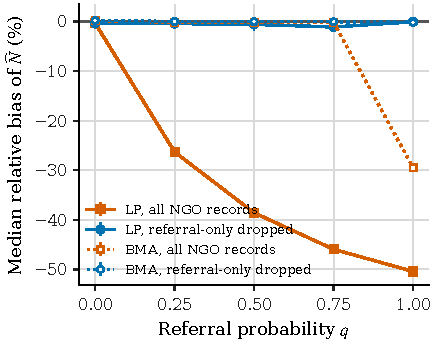
\includegraphics[width=2.9in]{figures/fig-sim-referral.pdf}
\end{minipage}\hfill
\begin{minipage}[b]{0.4\textwidth}
\caption{Synthetic data, S7 (independent capture, oracle linkage, $R=200$ per $q$). Median relative bias of $\Nhat$ against the referral probability $q$, using all NGO records or after dropping referral-only records by their provenance flag (\cref{prop:referral}(c)). Bars: $\pm2$ MCSE. Coverage is in \cref{tab:sim-referral}.}\label{fig:sim-referral}
\end{minipage}
\end{figure}

\begin{figure}[t]
\centering
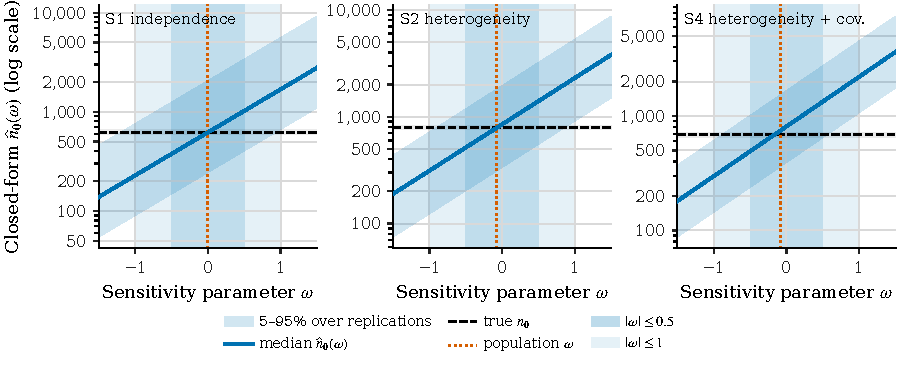
\includegraphics[width=6in]{figures/fig-sim-sensitivity.pdf}
\caption{Synthetic data, S6. Closed-form $\widehat n_{\zero}(\omega)$ on the oracle tables of S1, S2 and S4 ($R=100$): median curve and $5$--$95\%$ band over replicates, on a log scale. Shading: $|\omega|\le0.5$ and $|\omega|\le1$. Dashed: mean true $n_{\zero}$ (grey band: its $5$--$95\%$ range). Dotted: mean population $\omega$.}\label{fig:sim-sensitivity}
\end{figure}

\paragraph{(Q2) Sensitivity bands.} S6 applies the closed form \eqref{eq:id-closed} to the oracle tables (\cref{fig:sim-sensitivity}, \cref{tab:sim-sensitivity}). At $\omega=0$ its median error in $n_{\zero}$ is $-0.2\%$ (S1), $+4.1\%$ (S2), $-0.1\%$ (S3) and $+18.2\%$ (S4). The population top interaction is $0$ in S1 and S3, $-0.074$ in S2 and $-0.086$ in S4. For $K=4$, $\bar\omega=\omega$, so \cref{prop:direction} predicts that S2 and S4 overstate the dark figure, as they do. The asymptotic overstatement $e^{-\bar\omega}-1$ is $+7.7\%$ and $+9.0\%$, and the S4 median exceeds it.

The estimated bounds $[\widehat n_{\zero}(-\Omega),\widehat n_{\zero}(\Omega)]$ of \cref{cor:bounds}(b) contain $n_{\zero}$ in $87\%$ (S1), $93\%$ (S2), $87\%$ (S3) and $98\%$ (S4) of replicates for $\Omega=1$, and in $50$--$71\%$ for $\Omega=0.5$. These are point estimates of the identified set. They make no allowance for sampling error, and the closed form is noisy, so they can miss $n_{\zero}$ even when $|\omega|\le\Omega$ holds, as in S1 and S3. The union of the Wald intervals for $n_{\zero}$ over $|\omega|\le\Omega$ (the construction of \cref{cor:bounds}(c) with $c=z_{0.975}$) contains $n_{\zero}$ in $99$--$100\%$ of replicates for $\Omega=0.5$ and in $100\%$ for $\Omega=1$. The price is width. At $\Omega=1$ the bounds span a factor of $e^2\approx7.4$; the median bounds in S1 are $[228,1682]$, against a mean true $n_{\zero}$ of $622$. The bands therefore behave as the theory says. Without a substantive bound on $\omega$, however, they are too wide to inform policy. This is the identification problem of \cref{thm:nonid}, not a feature of the simulation.

\begin{figure}[t]
\centering
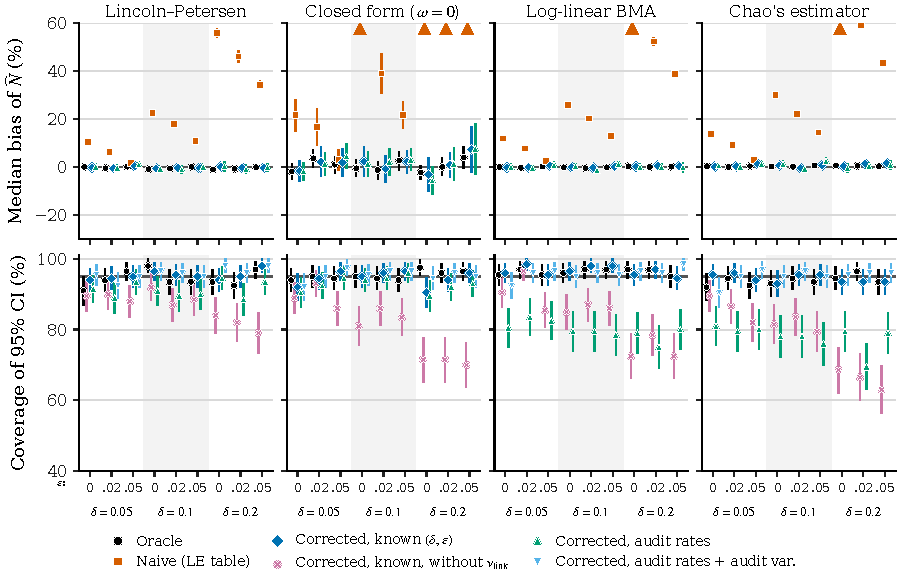
\includegraphics[width=6in]{figures/fig-sim-le-validation.pdf}
\caption{Synthetic data, S8: observed tables generated by the LE model (independent capture, $N=2000$, $R=200$ per $(\delta,\varepsilon)$ cell). Top: median relative bias of $\Nhat$ (bars $\pm2$ MCSE; triangles: off the axis). Bottom: coverage of nominal $95\%$ intervals (bars $\pm2$ MCSE). Known: correction with the true $(\delta,\varepsilon)$. Audit rates: rates from a simulated random audit (200 records, 100 linked edges).}\label{fig:sim-le-validation}
\end{figure}

\begin{table}[t]
\centering
\caption{Synthetic data, S8: the LE model generates the observed table (independent capture, $N=2000$, $R=200$ per cell; coverage MCSE about $1.5$ points). Naive: estimator applied to the LE table. Known: correction with the true $(\delta,\varepsilon)$. Audit: correction with audit-estimated rates (200 records, 100 linked edges). Known$^-$: interval without $v_{\mathrm{link}}$, as in the first run. Known and Audit: interval with $v_{\mathrm{link}}$. Audit$^+$: with the audit variance added.}\label{tab:sim-le}
\small
\setlength{\tabcolsep}{4pt}
\simfit{% Generated by code/make_figures.py from results/sim_results.json (run 2) -- do not edit by hand.
% S8: observed table = simulate_observed(t_true, delta, eps) (the LE model itself); independent capture,
% N = 2000, R = 200 per cell. Known: linkage_corrected with the true (delta, eps); Audit: rates from a
% random audit simulated from the LE ground truth (200 records + 100 linked edges). Known^-: interval without
% v_link (inner estimator only, as in run 1); Known/Audit: with v_link; Audit^+: + audit variance.
\begin{tabular}{@{}rrrrrrrrrrrrr@{}}
\toprule
 & & \multicolumn{3}{c}{BMA: median bias (\%)} & \multicolumn{5}{c}{BMA: coverage (\%)} & \multicolumn{3}{c}{Known rates: cov. with / without $v_{\mathrm{link}}$} \\
\cmidrule(lr){3-5}\cmidrule(lr){6-10}\cmidrule(lr){11-13}
$\delta$ & $\varepsilon$ & Naive & Known & Audit & Oracle & Known$^-$ & Known & Audit & Audit$^+$ & LP & CF & Chao \\
\midrule
0.05 & 0 & $+$11.9 & $-$0.2 & $-$0.1 & 96 & 90 & 96 & 80 & 92 & 94/90 & 92/89 & 96/90 \\
0.05 & 0.02 & $+$7.8 & $-$0.2 & $-$0.4 & 97 & 96 & 98 & 84 & 96 & 94/90 & 94/93 & 96/86 \\
0.05 & 0.05 & $+$2.4 & $+$0.5 & $+$0.8 & 96 & 86 & 96 & 82 & 96 & 95/88 & 96/86 & 94/82 \\
\addlinespace
0.1 & 0 & $+$25.9 & $-$0.1 & $+$0.1 & 96 & 85 & 96 & 80 & 95 & 96/92 & 95/81 & 93/82 \\
0.1 & 0.02 & $+$20.2 & $-$0.3 & $-$1.5 & 97 & 87 & 98 & 80 & 96 & 96/87 & 96/86 & 96/84 \\
0.1 & 0.05 & $+$12.9 & $+$0.1 & $+$1.1 & 97 & 86 & 98 & 78 & 96 & 95/88 & 96/84 & 96/80 \\
\addlinespace
0.2 & 0 & $+$62.7 & $+$0.2 & $-$0.1 & 97 & 72 & 96 & 79 & 96 & 94/84 & 90/72 & 94/68 \\
0.2 & 0.02 & $+$52.4 & $+$0.5 & $-$0.2 & 97 & 78 & 97 & 75 & 96 & 95/82 & 94/72 & 94/66 \\
0.2 & 0.05 & $+$38.9 & $+$0.3 & $-$0.3 & 95 & 72 & 94 & 80 & 98 & 98/79 & 96/70 & 94/63 \\
\bottomrule
\end{tabular}
}
\end{table}

\paragraph{(Q3) Does the LE correction work when its model holds?} Yes (S8; \cref{fig:sim-le-validation}, \cref{tab:sim-le}). Across the grid the naive BMA is biased by $+2.4\%$ to $+62.7\%$. The bias grows with $\delta$, and merging partly offsets it. With the true $(\delta,\varepsilon)$ the corrected estimators are median-unbiased: BMA lies between $-0.3\%$ and $+0.5\%$, LP between $-0.7\%$ and $+0.3\%$, Chao between $-0.4\%$ and $+1.5\%$, and the heavy-tailed closed form between $-3.2\%$ and $+7.3\%$. The intervals need $v_{\mathrm{link}}$. With it, BMA covers in $0.945$--$0.985$ of replicates, close to the oracle's $0.950$--$0.970$. Without it, as in the first run, BMA covers in only $0.725$--$0.965$, worst at $\delta=0.2$. LP and Chao behave alike: $0.940$--$0.980$ and $0.930$--$0.960$ with $v_{\mathrm{link}}$, and $0.790$--$0.920$ and $0.630$--$0.895$ without. The closed form drops to $0.905$ at $\delta=0.2$, $\varepsilon=0$, where its forward-difference gradient is inaccurate.

With audit-estimated rates the point estimates stay median-unbiased (BMA $-1.5\%$ to $+1.1\%$). The audit's own $95\%$ intervals cover the realised $\delta$ in $0.895$--$0.95$ of replicates and the realised $\varepsilon$ in $0.91$--$0.93$. However, $v_{\mathrm{link}}$ alone now undercovers (BMA $0.750$--$0.835$, Chao $0.695$--$0.810$), because it ignores the audit error. Adding the audit variance of \cref{cor:linkcorrect}(iii) restores coverage: BMA $0.925$--$0.985$, LP $0.925$--$0.980$, CF $0.920$--$0.975$ and Chao $0.905$--$0.970$. As \cref{rem:link-sameaudit} predicts, the sum is conservative in some cells. It is also costly: the median BMA width is $0.17N$--$0.44N$, against $0.12N$--$0.22N$ with known rates.

\begin{figure}[t]
\centering
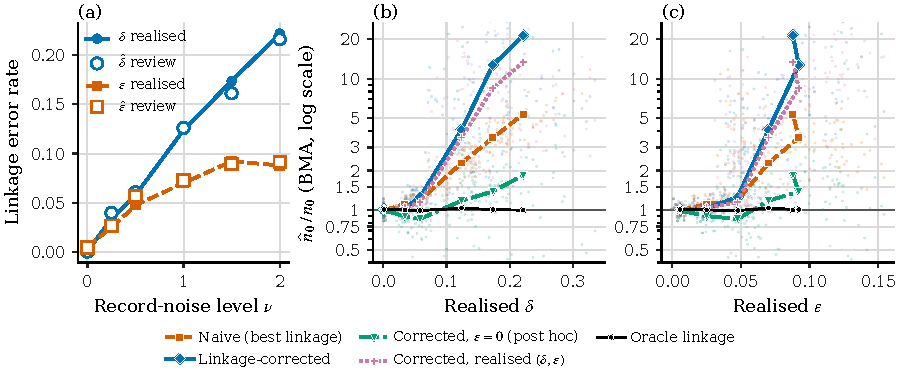
\includegraphics[width=6in]{figures/fig-sim-linkage-error.pdf}
\caption{Synthetic data, S5 (independent capture, record-noise sweep, $R=40$ per level). (a) Means over replicates of the realised capture-level rates $\delta$ and $\varepsilon$ of the point linkage, the same rates on the audit frame, and the audit estimates. (b, c) Dark-figure ratio $(\Nhat-n)/n_{\zero}$ for BMA against the realised $\delta$ and $\varepsilon$, on a log scale, where $n$ is the true number of recorded incidents. Points: replicates. Lines: medians by noise level. The $\varepsilon=0$ variant is post hoc.}\label{fig:sim-linkage-error}
\end{figure}

\begin{table}[t]
\centering
\caption{Synthetic data. BMA under realistic linkage: the S5 noise sweep (independent capture, $R=40$ per level) and S4 ($R=100$). Rates: means over replicates of the realised capture-level false-match rate $\varepsilon$ of the point linkage, its audit estimate $\hat\varepsilon$, and the best-fit $\varepsilon^\ast$. Remaining columns: median relative bias of $\Nhat$ in $\%$; the superscript counts replicates with $\Nhat>5N$. LE-corr.: audit rates. Realised: realised rates. $^\dagger$\,Post hoc variant, added after the first run. $^\ddagger$\,Infeasible diagnostic that uses the oracle table. Generated from \texttt{results/sim\_results.json}.}\label{tab:sim-realistic}
\small
\setlength{\tabcolsep}{4pt}
% Rows generated by a script from results/sim_results.json (run 2):
%   rates   = scenarios[S5|S4].results[i].linkage.{eps_true,eps_hat,lefit_eps}.mean
%   biases  = scenarios[...].estimates[pipeline].bma.relbias_median, pipelines
%             oracle, naive, corrected, corrected_true, corrected_d, corrected_lefit, mi
%   [k]     = estimates[pipeline].bma.n_blowup
\begin{tabular}{@{}lrrrrrrrrrr@{}}
\toprule
 & \multicolumn{3}{c}{False-match rate} & \multicolumn{7}{c}{Median relative bias of $\Nhat$ (\%)} \\
\cmidrule(lr){2-4}\cmidrule(lr){5-11}
 & $\varepsilon$ & $\hat\varepsilon$ & $\varepsilon^\ast$ & Oracle & Naive & LE-corr. & Realised & $\varepsilon{=}0^\dagger$ & Best-fit$^\ddagger$ & MI \\
\midrule
S5, $\nu=0$ & 0.006 & 0.006 & 0.010 & $+$0.7 & $\phantom{+}$0.0 & $+$0.4 & $+$0.8 & $-$0.2 & $+$0.5 & $+$0.1 \\
S5, $\nu=0.25$ & 0.025 & 0.023 & 0.011 & $+$0.3 & $+$4.5 & $+$1.5 & $+$1.8 & $-$3.1 & $-$0.3 & $+$8.7 \\
S5, $\nu=0.5$ & 0.048 & 0.051 & 0.015 & $-$0.2 & $+$7.2 & $+$7.5 & $+$4.5 & $-$5.0 & $-$0.7 & $+$17.1 \\
S5, $\nu=1$ & 0.070 & 0.072 & 0.008 & $+$0.6 & $+$40.4 & $+$63.4\textsuperscript{[1]} & $+$52.1 & $+$3.0 & $+$9.2 & $+$41.1 \\
S5, $\nu=1.5$ & 0.092 & 0.088 & 0.012 & $+$0.4 & $+$75.3 & $+$158.5\textsuperscript{[7]} & $+$219.7\textsuperscript{[5]} & $+$9.7 & $+$22.4 & $+$44.2 \\
S5, $\nu=2$ & 0.088 & 0.093 & 0.002 & $+$0.3 & $+$117.8 & $+$367.2\textsuperscript{[18]} & $+$306.9\textsuperscript{[14]} & $+$15.0 & $+$27.0 & $+$53.3 \\
\addlinespace
S4 & 0.077 & 0.079 & 0.000 & $-$7.5 & $+$40.0 & $+$47.1\textsuperscript{[1]} & $+$38.5 & $-$4.5 & $+$4.3 & $+$44.2 \\
\bottomrule
\end{tabular}
\end{table}

\paragraph{(Q4) Does it work under realistic linkage?} No (S4, S5; \cref{fig:sim-linkage-error}, \cref{tab:sim-realistic}). Take S4. The point linkage has pairwise precision $0.905$ and recall $0.787$. On average it misses $37.9$ of $91.6$ within-list duplicates and leaves $126.7$ more clusters than there are recorded incidents, so the naive BMA is $+40.0\%$ (coverage $0.07$). The audit estimates its targets well: $\hat\delta=0.107$ against $0.111$ on its frame, and $\hat\varepsilon=0.079$ against $0.081$, with interval coverage $0.96$ and $0.98$. Yet the LE-corrected BMA is $+47.1\%$ (mean $+75.3\%$, one blow-up), worse than naive. Its coverage is $0.24$, and $0.10$ without $v_{\mathrm{link}}$. With the audit variance, coverage rises to $0.76$, but only because the median interval is $2.36N$ wide. The corrected closed form is $+458.8\%$, with 54 blow-ups in 100 replicates.

The audit is not to blame. With the realised rates of the point linkage the correction still gives $+38.5\%$. What fails is the model. The best-fitting scalar LE has $\varepsilon^\ast=0.000$ in every S4 replicate (with $\delta^\ast=0.079$ on average), and in S5 its mean $\varepsilon^\ast$ lies between $0.002$ and $0.015$. Yet $7$--$9\%$ of singletons are falsely merged at $\nu\ge1$ and in S4.

The explanation is \emph{swaps}. Under the one-record-per-list constraint, a record whose true partner is degraded by noise is typically linked to a wrong partner from the same list. Suppose the true clusters are $\{a_1,a_2\}$ and $\{b_2\}$, where subscripts denote lists, and the linkage returns $\{a_1,b_2\}$ and $\{a_2\}$. The capture table is unchanged. LE has no move that links a record to the wrong partner. The audit, however, correctly counts this swap as one split true pair and one false edge, which raises both $\hat\delta$ and $\hat\varepsilon$. Inverting a merge rate that left no trace in the table then over-corrects. Missed duplicates add singletons that LE does not model either (\cref{rem:link-dedup}).

The S5 sweep shows the transition. At $\nu=0.25$ the correction helps ($+1.5\%$ against $+4.5\%$ naive). At $\nu=0.5$ it is neutral ($+7.5\%$ against $+7.2\%$). From $\nu=1$ on it is worse than naive: $+63.4\%$, $+158.5\%$ and $+367.2\%$, against $+40.4\%$, $+75.3\%$ and $+117.8\%$.

Two further pipelines bracket what is achievable. The $\varepsilon=0$ variant is the best feasible pipeline in the study: $-4.5\%$ with coverage $0.69$ in S4, and between $-5.0\%$ and $+15.0\%$ across S5. But we chose it after seeing the first run. It ignores false matches that the audit shows to be frequent, and it would be wrong whenever false matches do change the table, as they do in S8. We report it as a post hoc observation, not as a validated method. The infeasible best-fit LE gives $+4.3\%$ with coverage $0.93$ in S4. At $\nu=1$, $1.5$ and $2$, however, it gives $+9.2\%$, $+22.4\%$ and $+27.0\%$, and its minimised Pearson distance grows from $0.3$ at $\nu=0$ to $143$ at $\nu=2$ (S4: $35$). So at high noise not even the best scalar $(\delta,\varepsilon)$ can represent the errors.

The answer to Q4 is that the LE correction is a stylised forward model. It is valid when the errors are LE-like (Q3), and a random audit cannot by itself tell whether they are. A feasible way to diagnose this is to fit ``table-effective'' rates on audited clusters, the feasible analogue of $(\delta^\ast,\varepsilon^\ast)$, and compare them with $(\hat\delta,\hat\varepsilon)$. A large gap in $\varepsilon$ signals swap-dominated errors. We have not implemented this diagnostic.

\begin{table}[t]
\centering
\caption{Synthetic data. MI with Gibbs linkage draws (approximate posterior under the plug-in FS pairwise model) against the point linkage. False merges, pairwise recall over all records, and $n-n^\star$ (clusters minus true recorded incidents) are means over replicates; draw columns average the first 5 draws of each replicate. BMA bias and coverage as in \cref{tab:sim-main}. S4: $R=100$; S5: $R=40$ per level.}\label{tab:sim-mi}
\small
% Generated by code/make_figures.py from results/sim_results.json (run 2) -- do not edit by hand.
% MI with Gibbs linkage draws (approximate posterior under the plug-in FS pairwise model) vs the point
% linkage. False merges, recall (pairwise, all records) and n - n* (observed clusters minus true observed
% incidents): means over replicates (draw columns: mean over the first 5 draws per replicate).
\begin{tabular}{@{}lrrrrrrrrrr@{}}
\toprule
 & \multicolumn{2}{c}{False merges} & \multicolumn{2}{c}{Recall} & \multicolumn{2}{c}{$n-n^\star$} & \multicolumn{2}{c}{BMA median bias (\%)} & \multicolumn{2}{c}{Cov. (\%)} \\
\cmidrule(lr){2-3}\cmidrule(lr){4-5}\cmidrule(lr){6-7}\cmidrule(lr){8-9}\cmidrule(lr){10-11}
Scenario & Point & Draw & Point & Draw & Point & Draw & Naive & MI & Naive & MI \\
\midrule
S4 & 98 & 112 & 0.787 & 0.710 & $+$127 & $+$178 & $+$40.0 & $+$44.2 & 7 & 6 \\
S5, $\nu=0$ & 5 & 7 & 0.998 & 0.993 & $-$4 & $-$2 & $-$0.0 & $+$0.1 & 92 & 95 \\
S5, $\nu=0.25$ & 25 & 27 & 0.932 & 0.898 & $+$22 & $+$41 & $+$4.5 & $+$8.7 & 55 & 28 \\
S5, $\nu=0.5$ & 52 & 54 & 0.884 & 0.816 & $+$31 & $+$71 & $+$7.2 & $+$17.1 & 45 & 10 \\
S5, $\nu=1$ & 102 & 113 & 0.760 & 0.674 & $+$75 & $+$112 & $+$40.4 & $+$41.1 & 2 & 12 \\
S5, $\nu=1.5$ & 164 & 187 & 0.669 & 0.585 & $+$83 & $+$107 & $+$75.3 & $+$44.2 & 0 & 15 \\
S5, $\nu=2$ & 208 & 247 & 0.581 & 0.509 & $+$113 & $+$115 & $+$117.8 & $+$53.3 & 0 & 20 \\
\bottomrule
\end{tabular}

\end{table}

\paragraph{(Q5) Multiple imputation against the point linkage.} In S1--S3 the records are clean, and MI, naive and oracle agree (\cref{tab:sim-main}). Under noise MI does not beat the naive table except at the highest noise levels (\cref{tab:sim-mi}). In S4 the BMA is $+44.2\%$ under MI against $+40.0\%$ naive, with coverage $0.06$ and $0.07$. In S5, MI is worse at $\nu=0.25$ and $0.5$ ($+8.7\%$ against $+4.5\%$, and $+17.1\%$ against $+7.2\%$) and about equal at $\nu=1$ ($+41.1\%$ against $+40.4\%$). Only at $\nu=1.5$ and $2$ is it better ($+44.2\%$ against $+75.3\%$, and $+53.3\%$ against $+117.8\%$), and even there coverage is only $0.15$--$0.20$.

The reason is visible in the draws. They split more true clusters than the point linkage. In S4 their pairwise recall is $0.710$ against $0.787$, and they leave $177.6$ surplus clusters against $126.7$. MI therefore propagates uncertainty around a worse-centred table. This does not contradict \cref{prop:totalvar}(iv), which assumes exact draws from a correct linkage posterior; a plug-in, pairwise-composite target is neither. The sampler itself mixes quickly. In S4 the lag-1 autocorrelation of the number of links across sweeps is $-0.033$, and about $343$ of $2186$ active records change cluster in each sweep. The problem is the target, not the mixing. The Bernoulli-and-greedy imputation of the first run was worse ($+64.5\%$; \cref{tab:sim-run12}). We did not try a fully Bayesian linkage model, or calibrating $\pi$ on the audit sample.

\begin{table}[t]
\centering
\caption{Synthetic data. LCMCR convergence diagnostics for the oracle and naive tables (4 chains $\times$ 7500 iterations, burn-in 2500, thinning 5; overdispersed starting values). Diagnostics are for $N$: rank-normalised split-$\widehat R$ and bulk/tail ESS \citep{vehtari2021}. \% protocol: share of fits meeting \cref{app:comp-diag} ($\widehat R<1.01$, bulk and tail ESS $\ge400$). Bias and coverage in $\%$, MCSE in parentheses.}\label{tab:sim-lcmcr}
\setlength{\tabcolsep}{3pt}
\simfit{% Generated by code/make_figures.py from results/sim_results.json (run 2) -- do not edit by hand.
% LCMCR fits with 4 chains x 7500 iterations (2500 burn-in, thin 5; 4000 pooled draws), overdispersed n0 starts.
% Rank-normalised split-Rhat and bulk / tail ESS of N (Vehtari et al. 2021). % protocol: fits meeting App. app:comp-diag
% (Rhat < 1.01 and bulk and tail ESS >= 400). Bias and coverage in %, Monte Carlo SE in parentheses.
\begin{tabular}{@{}llrrrrrrrrrr@{}}
\toprule
Scen. & Table & Fits & $\widehat R$ med. & $\widehat R$ max & \% $\widehat R{<}1.01$ & ESS$_b$ med. & ESS$_b$ min & ESS$_t$ med. & \% protocol & Median bias (MCSE) & Cov. (MCSE) \\
\midrule
S1 & Oracle & 10 & 1.002 & 1.004 & 100 & 2848 & 1479 & 3239 & 100 & $-$1.2 (1.6) & 90 (9) \\
S1 & Naive & 10 & 1.001 & 1.031 & 90 & 2990 & 161 & 3198 & 80 & $-$1.4 (1.7) & 90 (9) \\
S2 & Oracle & 25 & 1.042 & 1.240 & 8 & 95 & 13 & 168 & 0 & $-$10.2 (1.1) & 88 (6) \\
S2 & Naive & 25 & 1.048 & 1.341 & 8 & 105 & 10 & 179 & 0 & $-$10.6 (1.4) & 88 (6) \\
S3 & Oracle & 10 & 1.018 & 1.232 & 10 & 234 & 13 & 243 & 10 & $-$2.3 (1.9) & 100 (0) \\
S3 & Naive & 10 & 1.008 & 1.033 & 60 & 407 & 145 & 700 & 40 & $-$2.1 (1.7) & 100 (0) \\
S4 & Oracle & 25 & 1.031 & 1.197 & 8 & 174 & 15 & 231 & 4 & $-$8.7 (0.8) & 88 (6) \\
S4 & Naive & 25 & 1.024 & 1.278 & 12 & 140 & 11 & 191 & 0 & $+$59.3 (5.0) & 4 (4) \\
\bottomrule
\end{tabular}
}
\end{table}

\paragraph{(Q6) LCMCR computation.} Each LCMCR fit uses four chains of 7500 iterations, with burn-in 2500 and thinning 5, from overdispersed starting values for $n_{\zero}$, giving 4000 pooled draws. \Cref{app:comp-diag} requires $\widehat R<1.01$ and bulk and tail effective sample sizes of at least 400. All S1 oracle fits meet this protocol, and $80\%$ of the S1 naive fits. The S2 and S4 fits do not (\cref{tab:sim-lcmcr}). Only $8$--$12\%$ of them reach $\widehat R<1.01$. Their median $\widehat R$ is $1.024$--$1.048$, with maxima up to $1.341$, and their median bulk ESS is $95$--$174$. Only $0$--$4\%$ meet the protocol, and in S3 $10\%$ (oracle) and $40\%$ (naive) do. The LCMCR results for S2--S4 therefore come from a reduced protocol and must be read as such. The corrected and MI fits pool one chain per imputation, so they have no $\widehat R$.

Two pieces of evidence suggest that the shortfall does not drive the reported biases. First, the four chain medians of a fit differ by a median of $2.9\%$ of $N$ in S2 (maximum $13.2\%$), about $2\%$ in S4 with oracle linkage (maximum $7.4\%$) and $5.9\%$ in S4 with naive linkage (maximum $20.6\%$). The first two are small next to the oracle biases of $-10.2\%$ and $-8.7\%$. Second, the first run, with single chains of 6000 iterations on 40 replicates, gave similar medians: $-11.2\%$ in S2 and $-8.3\%$ in S4 (\cref{tab:sim-run12}). This is evidence, not proof. LCMCR should not be used on real data until a run meets the protocol.

\subsection{What the simulation does and does not show}\label{sec:sim-scope}

The simulation shows four things. First, the identification results of \cref{sec:identification} hold in finite samples. Referral and heterogeneity bias Lincoln--Petersen by close to their population limits. Provenance recoding, or lists unconnected to the referral channel, remove the referral bias. Chao's estimator falls below $N$ under incident heterogeneity and slightly above it under list heterogeneity. Second, when LE holds, the correction of \cref{cor:linkcorrect} removes the bias, and its intervals are calibrated once $v_{\mathrm{link}}$ and the audit variance are included. Third, under realistic FS-EM linkage the same correction with well-estimated rates over-corrects, because the errors are dominated by swaps that scalar LE cannot represent. Fourth, multiple imputation from a plug-in pairwise posterior does not repair a biased linkage.

The simulation does not show the following.
\begin{itemize}
  \item It says nothing about real lists. The worlds are not calibrated to any source, and there is one population size ($N=2000$) and one number of lists ($K=4$). Calibration is part of the analysis plan (\cref{sec:plan}).
  \item It does not evaluate the fully Bayesian linkage of \cref{alg:pipeline}, with uncertain $m$ and $u$ and duplicates resolved jointly, nor the targeted review of \cref{alg:review}.
  \item It does not evaluate a feasible estimator of table-effective linkage rates.
  \item It does not evaluate the covariate, small-area and funnel models of \cref{sec:models-cov,sec:models-sae,sec:funnel}.
  \item Its LCMCR results for S2--S4 rest on a sampler that does not meet our own convergence protocol, and LCMCR is never refitted over a grid of $\omega$ or $q$.
\end{itemize}
The post hoc $\varepsilon=0$ variant performed best under realistic linkage, but nothing here licenses it as a default.
